% =====================================================================
%  Thesis Defense Presentation (short version, ~15 min)
%  Trading Under Uncertainty: A Meta-Verification Framework for
%  Machine Learning in Intraday Forex Trading
%
%  Compile from the ./thesis folder:  pdflatex Thesis_Presentation_Short.tex  then bibtex, then pdflatex twice
% =====================================================================
\documentclass[aspectratio=169, 11pt]{beamer}

\usepackage[utf8]{inputenc}
\usepackage[T1]{fontenc}
\usepackage{lmodern}
\usepackage{amsmath, amssymb, bm}
\usepackage{graphicx}
\usepackage{booktabs}
\usepackage{colortbl}
\usepackage{multicol}
\usepackage{tikz}
\usepackage{pgfplots}
\pgfplotsset{compat=1.17}
\usetikzlibrary{positioning, arrows.meta, shapes.misc, calc}

\graphicspath{{../data/figures/}}

% ---------------------------------------------------------------------
%  Colours (University of Bologna red + neutrals)
% ---------------------------------------------------------------------
\definecolor{unibored}{RGB}{187, 46, 41}
\definecolor{uniboreddark}{RGB}{140, 30, 28}
\definecolor{ink}{RGB}{38, 38, 42}
\definecolor{muted}{RGB}{110, 110, 118}
\definecolor{paper}{RGB}{248, 246, 244}
\definecolor{good}{RGB}{46, 125, 80}
\definecolor{bad}{RGB}{176, 58, 46}
\definecolor{neutralbar}{RGB}{160, 160, 168}

\setbeamercolor{normal text}{fg=ink}
\setbeamercolor{structure}{fg=unibored}
\setbeamercolor{alerted text}{fg=unibored}
\setbeamercolor{frametitle}{fg=ink}
\setbeamercolor{itemize item}{fg=unibored}
\setbeamercolor{itemize subitem}{fg=unibored!70}
\setbeamercolor{enumerate item}{fg=unibored}
\setbeamercolor{block title}{bg=unibored, fg=white}
\setbeamercolor{block body}{bg=paper, fg=ink}
\setbeamercolor{block title alerted}{bg=ink, fg=white}
\setbeamercolor{block body alerted}{bg=paper, fg=ink}
\setbeamercolor{block title example}{bg=good, fg=white}
\setbeamercolor{block body example}{bg=paper, fg=ink}

% ---------------------------------------------------------------------
%  Fonts & templates
% ---------------------------------------------------------------------
\usefonttheme{professionalfonts}
\renewcommand{\familydefault}{\sfdefault}
\setbeamerfont{frametitle}{size=\Large, series=\bfseries}
\setbeamerfont{block title}{series=\bfseries}

\setbeamertemplate{navigation symbols}{}
\setbeamertemplate{itemize items}[circle]
\setbeamertemplate{itemize subitem}[triangle]
\setbeamertemplate{enumerate items}[default]
\setbeamertemplate{blocks}[rounded][shadow=false]
\setbeamersize{text margin left=10mm, text margin right=10mm}

% Frame title: red accent bar + title + thin rule
\makeatletter
\setbeamertemplate{frametitle}{%
  \vspace*{4mm}%
  \begin{tikzpicture}[remember picture, overlay]
    \fill[unibored] ([yshift=-4mm]current page.north west) rectangle ++(3mm,-9mm);
  \end{tikzpicture}%
  \usebeamerfont{frametitle}\usebeamercolor[fg]{frametitle}\insertframetitle
  \ifx\insertframesubtitle\@empty\else
    \\[-1mm]{\normalsize\color{muted}\insertframesubtitle}%
  \fi
  \vspace*{-1mm}\par
  {\color{unibored!25}\rule{\linewidth}{0.6pt}}%
}
\makeatother

% Footline: author | short title | page
\setbeamertemplate{footline}{%
  \leavevmode%
  \begin{beamercolorbox}[wd=\paperwidth, ht=6mm, dp=2mm]{}%
    \hspace*{10mm}{\scriptsize\color{muted}\insertshortauthor\ \ \textbar\ \ \insertshorttitle}%
    \hfill%
    {\scriptsize\bfseries\color{unibored}\insertframenumber\,/\,\inserttotalframenumber}\hspace*{10mm}%
  \end{beamercolorbox}%
}

% Section divider
\AtBeginSection[]{%
  {\setbeamertemplate{footline}{}
  \begin{frame}[plain, noframenumbering]
    \begin{tikzpicture}[remember picture, overlay]
      \fill[unibored] (current page.south west) rectangle (current page.north east);
      \node[anchor=north west, text=white, font=\huge\bfseries, text width=130mm, align=left, inner sep=0pt]
        (sec) at ([xshift=10mm, yshift=0mm]current page.west) {\hyphenpenalty=10000\exhyphenpenalty=10000 \insertsectionhead};
      \node[anchor=south west, text=white, font=\fontsize{40}{40}\selectfont\bfseries, opacity=0.25, inner sep=0pt]
        at ([yshift=5mm]sec.north west) {\thesection};
      \draw[white, line width=1pt] ([yshift=-5mm]sec.south west) -- ++(30mm,0);
    \end{tikzpicture}
  \end{frame}}
}
\makeatletter
\def\thesection{\ifnum\c@section<10 0\fi\the\c@section}
\makeatother

% Helpers
\newcommand{\hl}[1]{\textcolor{unibored}{\textbf{#1}}}
\newcommand{\pos}[1]{\textcolor{good}{\textbf{#1}}}
\newcommand{\negv}[1]{\textcolor{bad}{\textbf{#1}}}
\newcommand{\kpi}[2]{%
  \begin{tikzpicture}
    \node[fill=paper, rounded corners=3pt, minimum width=2.9cm, minimum height=1.8cm, align=center]
      {{\Huge\bfseries\color{unibored}#1}\\[2mm]\footnotesize\color{muted}#2};
  \end{tikzpicture}}
\newcommand{\kpismall}[2]{%
  \begin{tikzpicture}
    \node[fill=paper, rounded corners=3pt, minimum width=2.6cm, minimum height=1.3cm, align=center]
      {{\LARGE\bfseries\color{unibored}#1}\\[1mm]\scriptsize\color{muted}#2};
  \end{tikzpicture}}

% ---------------------------------------------------------------------
%  Metadata
% ---------------------------------------------------------------------
\title[Trading Under Uncertainty]{Trading Under Uncertainty}
\subtitle{A Meta-Verification Framework for Machine Learning\\in Intraday Forex Trading}
\author[Adam Scheuerlein]{Adam Scheuerlein}
\date{Graduation Session: October 2026}

% =====================================================================
\begin{document}
% =====================================================================

% ---------------------------------------------------------------------
%  Cover
% ---------------------------------------------------------------------
{\setbeamertemplate{footline}{}
\begin{frame}[plain, noframenumbering]
  \begin{tikzpicture}[remember picture, overlay]
    % left white panel with logo, right red panel with title
    \fill[white] (current page.south west) rectangle (current page.north east);
    \fill[unibored] ([xshift=-95mm]current page.north east) rectangle (current page.south east);

    % logo
    \node[anchor=center] (logo) at ([xshift=33mm, yshift=8mm]current page.west)
      {\includegraphics[width=50mm]{cover_page.png}};

    % department / degree under logo
    \node[anchor=north, align=center, text=ink, font=\footnotesize] at ([yshift=-3mm]logo.south)
      {Department of Statistical Sciences\\``Paolo Fortunati''};
    \node[anchor=north, align=center, text=unibored, font=\small\bfseries] at ([yshift=-14mm]logo.south)
      {Second Cycle Degree\\M.Sc. Quantitative Finance};

    % title block on red
    \node[anchor=north west, text width=82mm, align=left, text=white]
      at ([xshift=-89mm, yshift=-14mm]current page.north east)
      {{\fontsize{24}{28}\selectfont\bfseries Trading Under\\Uncertainty}\\[4mm]
       {\large A Meta-Verification Framework for Machine Learning in Intraday Forex Trading}};

    \draw[white, line width=1pt] ([xshift=-89mm, yshift=-58mm]current page.north east) -- ++(25mm,0);

    % people
    \node[anchor=north west, text width=40mm, align=left, text=white, font=\footnotesize]
      at ([xshift=-89mm, yshift=-63mm]current page.north east)
      {\textbf{Candidate}\\Adam Scheuerlein};
    \node[anchor=north west, text width=42mm, align=left, text=white, font=\footnotesize]
      at ([xshift=-47mm, yshift=-63mm]current page.north east)
      {\textbf{Supervisors}\\Prof. Umberto Cherubini\\Prof. Maurizio Morini};

    % session
    \node[anchor=south west, text=white!85!unibored, font=\scriptsize]
      at ([xshift=-89mm, yshift=6mm]current page.south east)
      {Graduation Session: October 2026 \quad\textbar\quad Academic Year 2025/2026};
  \end{tikzpicture}
\end{frame}}

% ---------------------------------------------------------------------
\begin{frame}{Outline}
  \begin{columns}[T,onlytextwidth]
    \begin{column}{0.48\textwidth}
      \begin{enumerate}
        \setlength{\itemsep}{3mm}
        \item Motivation \& Research Question
        \item Framework \& Methodology
      \end{enumerate}
    \end{column}
    \begin{column}{0.48\textwidth}
      \begin{enumerate}
        \setcounter{enumi}{2}
        \setlength{\itemsep}{3mm}
        \item Results: Tournament, Production \& Experiment
        \item Conclusion
      \end{enumerate}
    \end{column}
  \end{columns}
  \vfill
  \begin{block}{The thesis in one sentence}
    The value of this ML trading pipeline in intraday FX lies less in predicting the market than in
    \hl{deciding when \emph{not} to trade}.
  \end{block}
\end{frame}

% =====================================================================
\section{Motivation \& Research Question}
% =====================================================================

\begin{frame}{Quantifying the Unknown}
  \begin{columns}[c,onlytextwidth]
    \begin{column}{0.50\textwidth}
      \begin{itemize}
        \setlength{\itemsep}{2.5mm}
        \item Intraday FX: \hl{vanishingly low signal-to-noise ratio} and non-stationary regimes
        \item Given a random walk with drift, an ML model will \emph{always} find something. Is it structure, or a ghost in the data?
        \item The gullible approach treats price series as a standard supervised learning problem
        \item This thesis: shift from \hl{point-estimate trading} to \hl{meta-verification}
      \end{itemize}
    \end{column}
    \begin{column}{0.46\textwidth}
      \footnotesize
      \begin{block}{1 \; Data-Mining Trap}
        Exhaustive HPO on many features finds \emph{stochastic flukes}, not alpha
      \end{block}
      \vspace{0.5mm}
      \begin{block}{2 \; Hard Thresholds}
        A classifier trades at $p_{\text{long}} = 50.01\%$ exactly like at $95\%$. Costs would erode the edge (if any).
      \end{block}
      \vspace{0.5mm}
      \begin{block}{3 \; Regime Blindness}
        One model for G10 majors \emph{and} emerging markets ignores different liquidity and volatility.
      \end{block}
    \end{column}
  \end{columns}
\end{frame}

\begin{frame}{Research Question \& Objectives}
  \begin{center}
    
\begin{tikzpicture}
      \node[fill=unibored, text=white, rounded corners=3pt, inner sep=3mm, text width=0.86\textwidth, align=center]
        {\large\bfseries Can we build an ML classifier that drives a Forex trading model successfully?};
    \end{tikzpicture}
  \end{center}
  \vspace{1mm}
  \small
  \begin{tabular}{@{}p{0.04\textwidth}p{0.34\textwidth}p{0.54\textwidth}@{}}
    \toprule
    & \textbf{Objective} & \textbf{Question} \\
    \midrule
    \hl{1} & Architecture efficacy & Which of six ML architectures performs \hl{the least bad} under purged, nested walk-forward validation? \\
    \hl{2} & Meta-machinery & Can M2 veto weak M1 trades, and does conformal-like calibration beat a fixed cut-off? \\
    \hl{3} & Discovery control & Can the deflated Sharpe ratio (DSR) separate luck from systematic alpha? \\
    \hl{4} & Feature anatomy & Which features give stable signals, and why? \\
    \hl{5} & Global vs.\ local & One global model with pair-specific guardrails. Does it work for Majors and EMs? \\
    \bottomrule
  \end{tabular}
\end{frame}

% =====================================================================
\section{Framework \& Methodology}
% =====================================================================

\begin{frame}{The Meta-Verification Framework}
  \framesubtitle{Every signal must survive a chain of adversarial checks before it is traded}
  \begin{center}
  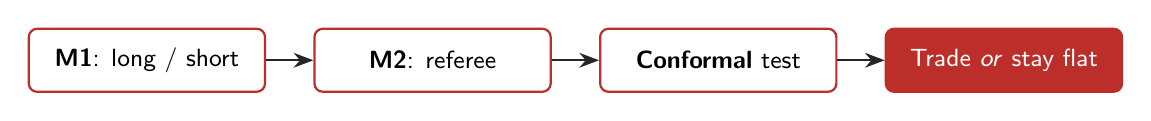
\begin{tikzpicture}[
      box/.style={draw=unibored, line width=0.8pt, rounded corners=3pt, minimum width=30mm,
                  minimum height=8mm, align=center, font=\small, fill=white},
      arr/.style={-{Stealth[length=2.5mm]}, line width=0.8pt, color=ink}]
    \node[box] (m1) {\textbf{M1}: long / short};
    \node[box, right=6mm of m1] (m2) {\textbf{M2}: referee};
    \node[box, right=6mm of m2] (cp) {\textbf{Conformal} test};
    \node[box, right=6mm of cp, fill=unibored, text=white] (tr) {Trade \emph{or} stay flat};
    \draw[arr] (m1) -- (m2);
    \draw[arr] (m2) -- (cp);
    \draw[arr] (cp) -- (tr);
  \end{tikzpicture}
  \end{center}
  \vspace{-1mm}
  \footnotesize
  \begin{columns}[T,onlytextwidth]
    \begin{column}{0.30\textwidth}
      \textbf{\small Triple-barrier labels}
      \[
        y_i = \begin{cases}
           1 & \text{TP first} \\
          -1 & \text{SL first} \\
          \operatorname{sgn}(r_i) & \text{time-out}
        \end{cases}
      \]
      Path-dependent labels: 146{,}711 in total (52.7\% short vs 47.3\% long).
    \end{column}
    \begin{column}{0.28\textwidth}
      \textbf{\small Meta-labels for M2}
      \[
        y_i^{\text{M2}} = \begin{cases}
          1 & \hat{y}_i^{\text{M1}} = y_i \\
          0 & \hat{y}_i^{\text{M1}} \neq y_i
        \end{cases}
      \]
      M1 picks the \emph{side}, M2 decides \emph{whether} to bet.
    \end{column}
    \begin{column}{0.36\textwidth}
      \textbf{\small Conformal veto}\; ($H_0$: \emph{signal is a mistake})
      \[
        p = \frac{\big|\{i : \alpha_i \geq \alpha_{\text{new}}\}\big| + 1}{k+1}
      \]
      \vspace{-3mm}
      \[
        \text{act} \iff p \leq \varepsilon
      \]
      $\alpha$ = M2 score\\
      calib. set = \hl{past M1 mistakes only}\\
      $\varepsilon$ bounds the Type-I error (with a caveat).
    \end{column}
  \end{columns}
  \vfill
  {\footnotesize\color{muted} FX data is not exchangeable \hl{(order matters)} $\Rightarrow$ the veto is more like a disciplined heuristic whose calibration is \emph{checked out-of-sample}.}
\end{frame}

\begin{frame}{An Effort to Guard Against False Discovery}
  \begin{columns}[c,onlytextwidth]
    \begin{column}{0.36\textwidth}
      \centering
      \includegraphics[height=0.66\textheight]{methodology/pipeline_structure.png}
    \end{column}
    \begin{column}{0.60\textwidth}
      \footnotesize
      \textbf{\small Purged, nested walk-forward}
      \begin{itemize}
        \item 2 outer $\times$ 2 inner folds: preprocessing \& feature selection once per outer fold
        \item Drop training obs.\ whose label window $[t_i, t_i + h_i]$ overlaps a test label
        \item Global test set touched \hl{exactly once}, by the tournament winner
      \end{itemize}
      \vspace{1mm}
      \textbf{\small Deflated Sharpe ratio}
      \vspace{-1mm}
      \[
        \text{DSR} = \Phi\!\left[\frac{(\widehat{SR} - SR^*)\sqrt{T-1}}{\sqrt{1 - \gamma_3\widehat{SR} + \frac{\gamma_4 - 1}{4}\widehat{SR}^2}}\right]
      \]
      \vspace{-2mm}
      \begin{itemize}
        \item $SR^*$ = best Sharpe expected \emph{by chance} after $N$ trials
          ($N$ = 1{,}250 per model \& fold. 5{,}000 in production)
        \item DSR $< 50\%$ $\Rightarrow$ indistinguishable from search luck
      \end{itemize}
    \end{column}
  \end{columns}
\end{frame}

\begin{frame}{Research Pipeline \& Experimental Design}
  \begin{columns}[c,onlytextwidth]
    \begin{column}{0.60\textwidth}
      \centering
      \includegraphics[width=\textwidth]{methodology/Methodology Flowchart.png}
    \end{column}
    \begin{column}{0.36\textwidth}
      \scriptsize
      \begin{itemize}
        \setlength{\itemsep}{1.2mm}
        \item \textbf{Data}: 11 pairs, hourly, 2024--2026, 7 Majors \& 4 EMs
        \item \textbf{94 features} $\to$ one common set per fold (correlation, MI, permutation importance)
        \item \textbf{Six M1 candidates}: RF, ExtraTrees, XGBoost, LightGBM, LSTM, GRU
        \item \textbf{M2 model}: RandomForest
        \item \textbf{Nested Optuna HPO}: models (outer), per-pair trading params (inner)
      \end{itemize}
    \end{column}
  \end{columns}
\end{frame}

% =====================================================================
\section{Results}
% =====================================================================

\begin{frame}{Tournament: Choosing the Least Fragile Architecture}
  \framesubtitle{Mean across 11 pairs and 2 outer folds}
  \centering
  \footnotesize
  \renewcommand{\arraystretch}{1.1}
  \resizebox{\textwidth}{!}{%
  \begin{tabular}{lcccccc}
    \toprule
    & RF & ExtraTrees & \cellcolor{unibored!12}\textbf{XGBoost} & LightGBM & LSTM & GRU \\
    \midrule
    Sharpe Ratio ($\pm$ std)  & $0.72 \pm 4.65$ & $0.57 \pm 4.87$ & \cellcolor{unibored!12}$\mathbf{1.97 \pm 4.50}$ & $1.18 \pm 4.49$ & $1.27 \pm 4.92$ & $1.53 \pm 5.12$ \\
    Deflated Sharpe (\% $\pm$ std)      & $27.22 \pm 39.04$ & $25.56 \pm 37.88$ & \cellcolor{unibored!12}$27.36 \pm 37.45$ & $\mathbf{32.6 \pm 38.99}$ & $29.98 \pm 36.27$ & $25.42 \pm 35.55$ \\
    Accepted-signal accuracy (\%, fold 1 / 2) & 57.2 / 68.7 & 56.5 / 72.8 & \cellcolor{unibored!12}58.3 / \textbf{74} & 57.5 / 70.3 & 56.8 / 63.6 & 58.6 / 68.7 \\
    Emp.\ FPR / $\varepsilon$ (fold 1 / 2) & \negv{2.23} / 0.87 & \negv{2.26} / 0.47 & \cellcolor{unibored!12}\pos{1.03} / 0.42 & 1.22 / 0.53 & \negv{2.30} / \negv{1.10} & \negv{1.64} / 0.70 \\
    \bottomrule
  \end{tabular}}
  \vspace{4mm}

  \begin{columns}[c,onlytextwidth]
    \begin{column}{0.30\textwidth}
      \centering\kpi{XGBoost}{Reciprocal Rank Fusion\\winner (score 0.19)}
    \end{column}
    \begin{column}{0.66\textwidth}
      \small
      \begin{itemize}
        \setlength{\itemsep}{1mm}
        \item Only XGBoost's veto stays close to its \hl{calibrated $\varepsilon$} (ratio $\approx 1$) and 4 of 6 let through $\sim$2$\times$ the mistakes in fold 1
        \item Veto sharpens as the calibration memory grows (at the price of low recall)
        \item Std.\ $>$ 2$\times$ mean: \textbf{no} architecture is uniformly profitable and the win is \emph{relative}
      \end{itemize}
    \end{column}
  \end{columns}
\end{frame}

\begin{frame}{What Actually Creates Value?}
  \framesubtitle{One building block at a time (XGBoost, avg.\ annualized Sharpe across 11 pairs)}
  \vspace{-1mm}
  \begin{center}
  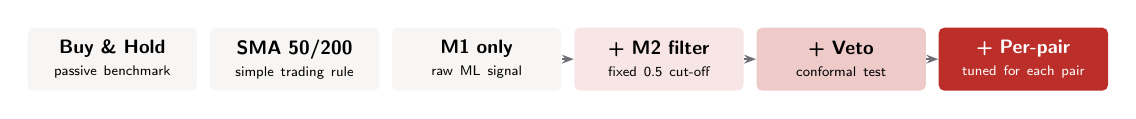
\begin{tikzpicture}[
      s/.style={rounded corners=2pt, minimum height=8mm, align=center, font=\scriptsize, inner sep=0.5mm, text width=20.5mm},
      arr/.style={-{Stealth[length=1.5mm]}, line width=0.6pt, color=muted}]
    \node[s, fill=paper] (a) {\textbf{Buy \& Hold}\\{\tiny passive benchmark}};
    \node[s, fill=paper, right=1.5mm of a] (b) {\textbf{SMA 50/200}\\{\tiny simple trading rule}};
    \node[s, fill=paper, right=1.5mm of b] (c) {\textbf{M1 only}\\{\tiny raw ML signal}};
    \node[s, fill=unibored!12, right=1.5mm of c] (d) {\textbf{+ M2 filter}\\{\tiny fixed 0.5 cut-off}};
    \node[s, fill=unibored!25, right=1.5mm of d] (e) {\textbf{+ Veto}\\{\tiny conformal test}};
    \node[s, fill=unibored, text=white, right=1.5mm of e] (f) {\textbf{+ Per-pair}\\{\tiny tuned for each pair}};
    \draw[arr] (c) -- (d); \draw[arr] (d) -- (e); \draw[arr] (e) -- (f);
  \end{tikzpicture}
  \end{center}
  \vspace{-2mm}
  \begin{columns}[c,onlytextwidth]
    \begin{column}{0.62\textwidth}
      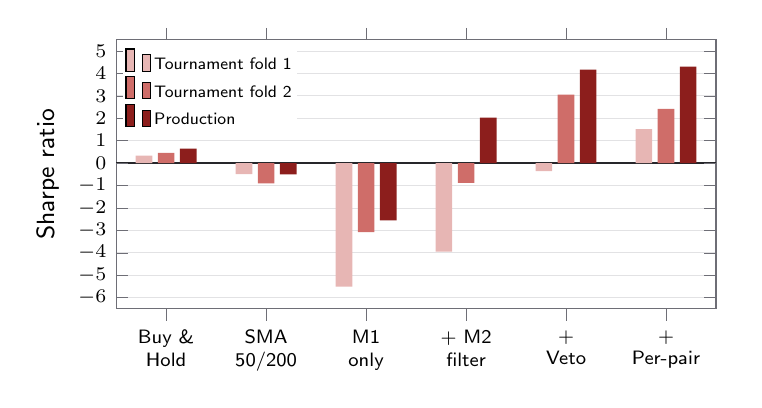
\begin{tikzpicture}
        \begin{axis}[
            ybar, width=9.2cm, height=5.0cm,
            bar width=6pt,
            symbolic x coords={B\&H, SMA, M1 Only, M1+M2 Fixed, M1+M2 Global, M1+M2 Conformal},
            xtick=data,
            xticklabels={Buy \&\\Hold, SMA\\50/200, M1\\only, + M2\\filter, +\\Veto, +\\Per-pair},
            x tick label style={font=\scriptsize, align=center, text width=15mm},
            ticklabel style={font=\scriptsize},
            ymin=-6.5, ymax=5.5,
            ytick={-6,-5,...,5},
            ymajorgrids, major grid style={muted!20, line width=0.3pt},
            ylabel={Sharpe ratio}, ylabel style={font=\small},
            enlarge x limits=0.1,
            legend cell align=left,
            legend style={at={(0.01,0.98)}, anchor=north west, font=\fontsize{6}{7}\selectfont, draw=none, fill=white, inner sep=1pt,
                          nodes={inner sep=1pt}},
            axis line style={muted}, major tick style={muted},
            extra y ticks={0}, extra y tick labels={},
            extra y tick style={grid=major, major grid style={ink, line width=0.6pt}},
          ]
          \addplot[fill=unibored!35, draw=none] coordinates
            {(B\&H,0.34) (SMA,-0.49) (M1 Only,-5.50) (M1+M2 Fixed,-3.94) (M1+M2 Global,-0.36) (M1+M2 Conformal,1.52)};
          \addplot[fill=unibored!70, draw=none] coordinates
            {(B\&H,0.46) (SMA,-0.90) (M1 Only,-3.08) (M1+M2 Fixed,-0.88) (M1+M2 Global,3.05) (M1+M2 Conformal,2.42)};
          \addplot[fill=uniboreddark, draw=none] coordinates
            {(B\&H,0.65) (SMA,-0.50) (M1 Only,-2.55) (M1+M2 Fixed,2.03) (M1+M2 Global,4.17) (M1+M2 Conformal,4.30)};
          \legend{Tournament fold 1, Tournament fold 2, Production}
        \end{axis}
      \end{tikzpicture}
    \end{column}
    \begin{column}{0.34\textwidth}
      \footnotesize
      \begin{itemize}
        \setlength{\itemsep}{0.5mm}
        \item \negv{Raw M1 is harmful}: worse than doing nothing
        \item M2 filter helps, but stays negative in the tournament
        \item \pos{Conformal veto} is profitable in all three windows
        \item Per-pair vs.\ shared settings: \emph{inconsistent}
      \end{itemize}
      \vspace{0.5mm}
      $\Rightarrow$ profit comes from \hl{refusing} trades, not from \emph{improving} them
    \end{column}
  \end{columns}
\end{frame}

\begin{frame}{Production: A very Concentrated Result}
  \framesubtitle{Global XGBoost refit, tested once on the untouched $\sim$11-week window}
  \begin{columns}[T,onlytextwidth]
    \begin{column}{0.44\textwidth}
      \centering
      \footnotesize
      \setlength{\tabcolsep}{3pt}
      \begin{tabular}{l|rrrr}
        \toprule
        Pair & Ret.\,\% & Sharpe & DSR\,\% & Trades \\
        \midrule
        USDZAR & 81.95 & 16.32 & 100.0 & 934 \\
        USDMXN & 17.38 & 14.45 & 100.0 & 947 \\
        USDTRY & 8.10 & 11.83 & 99.99 & 1019 \\
        USDCNH & 1.67 & 3.13 & \negv{39.56} & 730 \\
        \midrule
        EURUSD & 0.59 & 3.86 & 54.45 & 8 \\
        USDJPY & $-0.81$ & $-2.30$ & \negv{0.31} & 184 \\
        \textit{5 majors} & 0.00 & 0.00 & -- & \negv{0} \\
        \bottomrule
      \end{tabular}

      \vspace{0.5mm}
      {\scriptsize\color{muted} EMs above the line, majors below. DSR undefined without trades}
      \vspace{3mm}

      \raggedright
      \footnotesize
      Majors' $\varepsilon$ is a quantile of a \hl{pooled, EM-dominated} calibration set:
      \textbf{no potential edge, or just a different score scale?}
    \end{column}
    \begin{column}{0.51\textwidth}
      \begin{alertblock}{Red flags}
        \footnotesize
        \begin{itemize}
          \setlength{\itemsep}{0.8mm}
          \item Avg.\ Sharpe \hl{4.30} beats both tournament folds (1.52, 2.42), annualized from 11 weeks
          \item \hl{5 of 7 majors} never trade and ZAR, MXN, TRY give \hl{90\%} of summed Sharpes
          \item DSR $<$ 50\%: \hl{USDCNH} and \hl{USDJPY}; EURUSD borderline (54\%, only 8 trades)
          \item DSR rules out search luck, \emph{not} bad data: USDZAR may profit from \hl{flash crashes} no other source confirms
        \end{itemize}
      \end{alertblock}
    \end{column}
  \end{columns}
\end{frame}

\begin{frame}{Experiment: Pair-Specific Calibration}
  \framesubtitle{Only the calibration set changes: each pair vs.\ its \emph{own} past mistakes}
  \begin{columns}[c,onlytextwidth]
    \begin{column}{0.54\textwidth}
      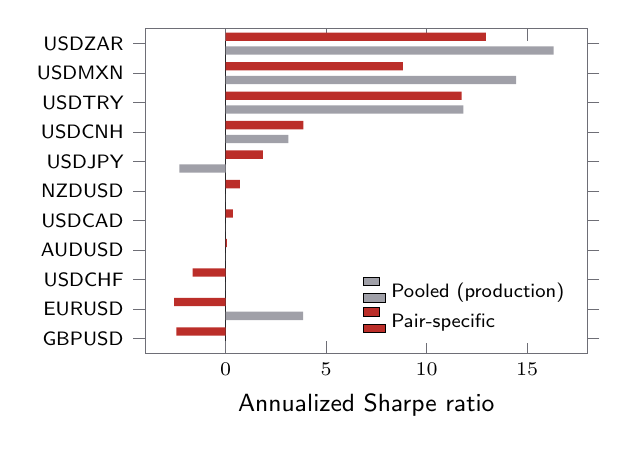
\begin{tikzpicture}
        \begin{axis}[
            xbar, width=7.2cm, height=5.7cm,
            legend cell align=left,
            bar width=3.0pt,
            symbolic y coords={USDZAR, USDMXN, USDTRY, USDCNH, USDJPY, NZDUSD, USDCAD, AUDUSD, USDCHF, EURUSD, GBPUSD},
            ytick=data, y dir=reverse,
            enlarge y limits=0.05,
            xmin=-4, xmax=18,
            ticklabel style={font=\scriptsize},
            xlabel={Annualized Sharpe ratio}, xlabel style={font=\small},
            legend style={at={(0.98,0.03)}, anchor=south east, font=\scriptsize, draw=none, fill=white},
            axis line style={muted}, major tick style={muted},
            extra x ticks={0}, extra x tick labels={},
            extra x tick style={grid=major, major grid style={ink, line width=0.6pt}},
          ]
          \addplot[fill=neutralbar, draw=none] coordinates
            {(16.32,USDZAR) (14.45,USDMXN) (11.83,USDTRY) (3.13,USDCNH) (-2.30,USDJPY) (0,NZDUSD) (0,USDCAD) (0,AUDUSD) (0,USDCHF) (3.86,EURUSD) (0,GBPUSD)};
          \addplot[fill=unibored, draw=none] coordinates
            {(12.94,USDZAR) (8.82,USDMXN) (11.74,USDTRY) (3.87,USDCNH) (1.85,USDJPY) (0.71,NZDUSD) (0.36,USDCAD) (0.06,AUDUSD) (-1.64,USDCHF) (-2.56,EURUSD) (-2.44,GBPUSD)};
          \legend{Pooled (production), Pair-specific}
        \end{axis}
      \end{tikzpicture}
    \end{column}
    \begin{column}{0.43\textwidth}
      \footnotesize
      \begin{itemize}
        \setlength{\itemsep}{0.8mm}
        \item \pos{USDJPY} $-2.30 \to +1.85$: pooling \emph{hid} a potential edge
        \item \negv{GBP, EUR, CHF} now lose: pooling was an \emph{accidental safeguard}
        \item USDCHF: same $\varepsilon = 0.02$, yet $0 \to 77$ trades
        \item Avg.\ Sharpe \hl{$4.30 \to 3.06$} ($\approx -30\%$): part of the production result is a \emph{calibration artifact}
      \end{itemize}
      \vspace{1mm}
      \begin{alertblock}{How real is any of it?}
        \scriptsize
        11 weeks is far too short to judge a trading strategy: 
        a few lucky trades can produce a Sharpe of 4.3. These results show promise, not proof.
      \end{alertblock}
    \end{column}
  \end{columns}
\end{frame}

% =====================================================================
\section{Conclusion}
% =====================================================================

\begin{frame}{Answering the Five Objectives}
  \small
  \renewcommand{\arraystretch}{1.25}
  \begin{tabular}{@{}p{0.03\textwidth}p{0.22\textwidth}p{0.08\textwidth}p{0.6\textwidth}@{}}
    \toprule
    & \textbf{Objective} & \textbf{Verdict} & \textbf{Evidence} \\
    \midrule
    \hl{1} & Architecture & \pos{Partial} & XGBoost is the least fragile under a shared protocol, which is a comparative, not absolute, win \\
    \hl{2} & Meta-machinery & \pos{Yes} & Raw M1 destroys value: the conformal veto is the load-bearing component as it it \emph{refuses} rather than \emph{improves} trades \\
    \hl{3} & DSR & \pos{Partial} & Flags USDCNH \& USDJPY (EURUSD borderline), but is blind to regime, tail and data risk (USDZAR) \\
    \hl{4} & Features & \pos{Partial} & Small stable core (VWMA, A/D, spread \& volatility), whereas the rest reshuffles across folds \\
    \hl{5} & Global vs.\ local & \negv{Open} & Per-pair vs.\ shared params (Kelly, SL/TP, $\varepsilon$, etc.): wins fold 1, loses fold 2. Per-pair $\varepsilon$ decides \emph{whether} a pair trades. Pooling hid USDJPY's edge \emph{and} shielded losing majors \\
    \bottomrule
  \end{tabular}
\end{frame}

\begin{frame}{Conclusion \& Outlook}
  \begin{columns}[c,onlytextwidth]
    \begin{column}{0.56\textwidth}
      \begin{itemize}
        \setlength{\itemsep}{2mm}
        \item A \textbf{raw classifier cannot} drive a profitable intraday FX strategy
        \item Embedded in meta-labeling + conformal veto, it \textbf{can} be made profitable on a \emph{subset} of pairs
        \item Profit comes from \hl{principled abstention}, not better directional accuracy
        \item Remaining edge is concentrated, event-dependent and fragile:
          a \emph{proof of concept} for the framework, not a deployable system
      \end{itemize}
    \end{column}
    \begin{column}{0.40\textwidth}
      \begin{block}{Next steps}
        \small
        \begin{itemize}
          \setlength{\itemsep}{2mm}
          \item CPCV for more backtest paths
          \item A single institutional data feed
          \item Exogenous macro features
          \item Modular refactor of the codebase
        \end{itemize}
      \end{block}
    \end{column}
  \end{columns}
\end{frame}

\begin{frame}{Explore the Code}
  \begin{columns}[c,onlytextwidth]
    \begin{column}{0.52\textwidth}
      \large
      The full pipeline is open source:
      \vspace{3mm}

      \normalsize
      \begin{itemize}
        \setlength{\itemsep}{2mm}
        \item Data aggregation \& sanity checks
        \item Feature engineering \& triple-barrier labelling
        \item Architecture tournament, M1/M2 meta-labeling \& conformal veto
        \item Custom backtester \& all result figures
      \end{itemize}
      \vspace{4mm}

      {\color{muted}\small github.com/adamwetzli/master\_thesis}
    \end{column}
    \begin{column}{0.42\textwidth}
      \centering
      \begin{tikzpicture}
        \node[fill=paper, rounded corners=4pt, inner sep=4mm, align=center] {%
          
\includegraphics[width=42mm]{./github qr code.png}\\[3mm]
          {\small\bfseries\color{unibored} Scan to open the repository}};
      \end{tikzpicture}
    \end{column}
  \end{columns}
\end{frame}

% ---------------------------------------------------------------------
%  Closing
% ---------------------------------------------------------------------
{\setbeamertemplate{footline}{}
\begin{frame}[plain, noframenumbering]
  \begin{tikzpicture}[remember picture, overlay]
    \fill[white] (current page.south west) rectangle (current page.north east);
    \fill[unibored] ([xshift=-95mm]current page.north east) rectangle (current page.south east);
    \node at ([xshift=33mm]current page.west) {\includegraphics[width=50mm]{cover_page.png}};
    \node[anchor=west, text=white, align=left] at ([xshift=-85mm, yshift=6mm]current page.east)
      {{\fontsize{30}{34}\selectfont\bfseries Thank you}\\[4mm]
       {\Large Questions \& discussion}};
    \draw[white, line width=1pt] ([xshift=-85mm, yshift=-12mm]current page.east) -- ++(25mm,0);
    \node[anchor=north west, text=white, font=\small, align=left] at ([xshift=-85mm, yshift=-16mm]current page.east)
      {Adam Scheuerlein\\M.Sc. Quantitative Finance --- University of Bologna};
  \end{tikzpicture}
\end{frame}}

% ---------------------------------------------------------------------
%  Bibliography (all entries of references.bib)
% ---------------------------------------------------------------------
\setbeamertemplate{bibliography item}[text]
\setbeamercolor{bibliography entry author}{fg=ink}
\setbeamercolor{bibliography entry title}{fg=ink}
\setbeamercolor{bibliography entry location}{fg=muted}
\setbeamercolor{bibliography entry note}{fg=muted}
\makeatletter
\def\beamer@newblock{\unskip\space}% keep each entry on running lines
\makeatother
{\setbeamertemplate{footline}{}
\begin{frame}[t, noframenumbering]{References}
  \nocite{*}
  \fontsize{4.5}{5.3}\selectfont
  \vspace*{-3mm}
  \setlength{\columnsep}{4mm}
  \begin{multicols}{4}
    \setlength{\itemsep}{0.5pt}
    \setlength{\parskip}{0pt}
    \bibliographystyle{plain}
    \bibliography{../data/bibliography/references}
  \end{multicols}
\end{frame}}

\end{document}
